%%%%%%%%%%%%%%%%%%%%%%%%%%%%%%%%%%%%%%%%%%%%%%%%%%%%%%%%%%%%%%%%%%%%%%%
\begingroup
\renewcommand{\cleardoublepage}{}
\renewcommand{\clearpage}{}
\vspace{1em}
\chapter{Исследовательские испытания}
\endgroup
%%%%%%%%%%%%%%%%%%%%%%%%%%%%%%%%%%%%%%%%%%%%%%%%%%%%%%%%%%%%%%%%%%%%%%%

\section{Испытания АПК}
Для проверки работоспособности изготовленного образца АПК сбора параметров прототип был установлен в серверную стойку лаборатории НИЛ АСПОД СПБПУ. Методика исследовательских испытаний предполагает сбор климатических параметров в течение трех месяцев с периодичностю раз в 4 часа. Результаты испытаний описаны ниже.
 
\begin{table}
	\captionsetup{skip=5pt}
	\caption{Результаты мониторинга параметров с использованием АПК}
	\centering
	\includegraphics[width=\textwidth]{resultTable}
	\label{tab:result}
\end{table}

Характер  изменения влажности  за  весь  период  наблюдения  приведен в табл. ~\ref{fig:humid}.

\begin{figure}[h]
	\centering
	\includegraphics[width=4.0in]{humid}
	\caption{График изменения влажности за весь период наблюдения}
	\label{fig:humid}
\end{figure}

Изменение  атмосферного давления  на протяжении периода мониторинга приведено на рис. ~\ref{fig:press}

 \begin{figure}[h]
 	\centering
 	\includegraphics[width=4.0in]{press}
 	\caption{График изменения давления за весь период наблюдения}
 	\label{fig:press}
 \end{figure}

Датчики  температуры  располагались  симметрично  на  передней  и задней стенках серверной стойки сверху и снизу блока.Наибольшая  температура  наблюдается  на  задней  стенке  стойки (красный и желтый графики),  при этом датчики, расположенные сверху задней стенки блока, также показывают большее  значение.  Изменение  температуры  на  протяжении  периода 
мониторинга приведено на рис. ~\ref{fig:temp}.

\begin{figure}[H]
	\centering
	\includegraphics[width=4.0in]{temper}
	\caption{Объединенный график изменения температуры за весь период наблюдения}
	\label{fig:temper}
\end{figure}
Вибрация  измерялась  как  интегрированное  значение  амплитуды колебаний за последние 100 мс до момента измерения. График измерения вибрации представлен на рис.  ~\ref{fig:vibr}.

\begin{figure}[!h]
	\centering
	\includegraphics[width=4.0in]{vibr}
	\caption{График изменения вибрации за весь период наблюдения}
	\label{fig:vibr}
\end{figure}

\begin{figure}[!h]
	\centering
	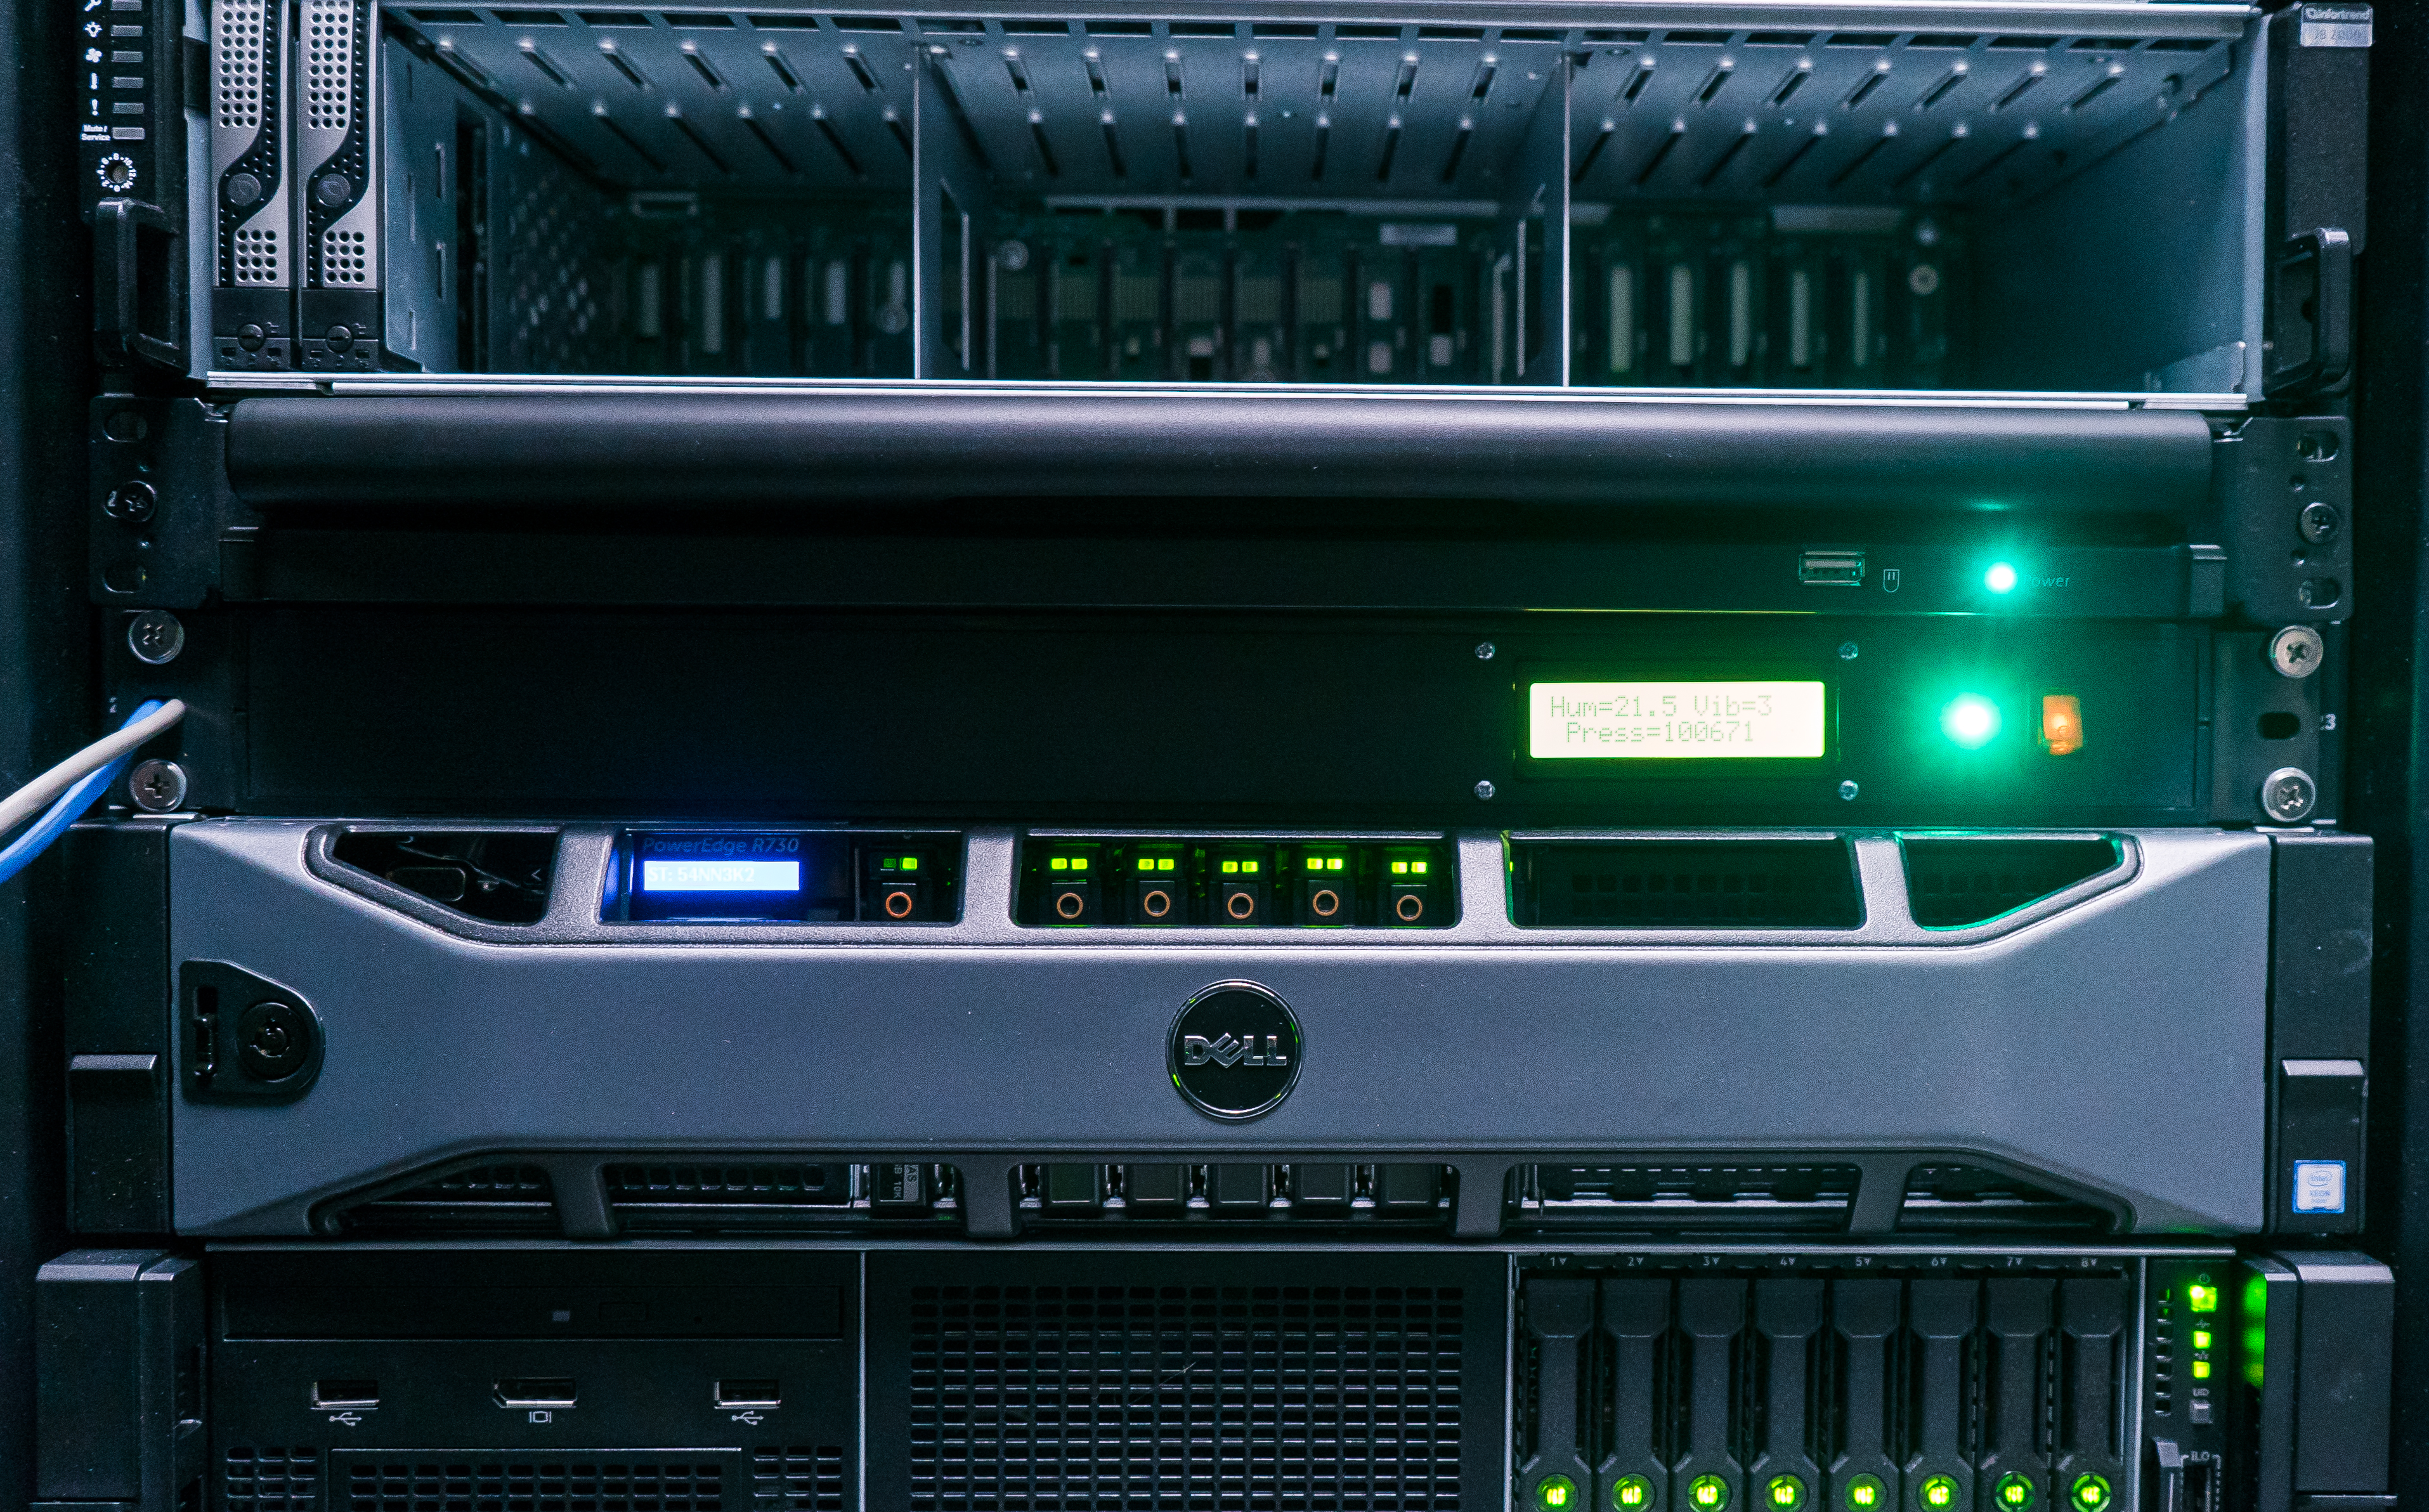
\includegraphics[width=4.0in]{inRack}
	\caption{Испытания комплекса в серверной}
	\label{fig:inRack}
\end{figure}

На графиках видно, что с 40 по 70 измерения происходит увеличение параметров влажности, вибрации и температуры одного из четырех датчиков (Т4), однако изменений в SMART параметрах дисков в серверной замечено не было.


На рис. ~\ref{fig:paramsRack} представлены данные,отображаемые на LCD дисплее.

\begin{figure}[!h]
	\centering
	\includegraphics[width=4.0in]{paramsRack}
	\caption{Показания LCD дисплея при испытаниях}
	\label{fig:paramsRack}
\end{figure}
За все время экспериментов диски в серверной не выходили из строя(находились в работоспособном состоянии), однако повышение уровня  вышупомянутых параметров повышает вероятность перехода в предотказное состояние. 

Таким образом, были проведены исследовательские испытания АПК в реальных условиях. На рис. ~\ref{fig:inRack} представлен АПК в серверной стойке.